\documentclass{beamer}

\usepackage{txfonts}
\usepackage{hyperref}
\usepackage{fancybox}
\usepackage{xfrac}
\usepackage{cancel}

\newcommand{\heart}{\ensuremath\heartsuit}

\usepackage{mathtools,amssymb}
\newcommand{\myarrow}{\scalebox{2}[2]{$\mathclap{\curvearrowleft}\mkern2.2mu
                                                 \mathclap{\curvearrowright}$}}

\DeclareMathOperator{\Bin}{\mathrm{Bin}}

\hypersetup{colorlinks=false,linkbordercolor=red,linkcolor=green,pdfborderstyle={/S/U/W 1}}

\addtobeamertemplate{navigation symbols}{}{ \hspace{1em}    \usebeamerfont{footline}%
    \insertframenumber / \inserttotalframenumber}

\geometry{papersize={15cm,13cm}}
\usepackage{lipsum}

\makeatletter
\newenvironment<>{contdproof}[1][\proofname]{%
    \par
    \def\insertproofname{#1\@addpunct{.}}%
    \usebeamertemplate{proof begin}#2}
  {\usebeamertemplate{proof end}}
\makeatother


\setbeamertemplate{theorems}[numbered]

\newtheorem*{nonumdefinition}{Definition}
\newtheorem*{nonumproblem}{Problem}
\newtheorem*{nonumtheorem}{Theorem}
\newtheorem*{nonumremark}{Remark}
\newtheorem*{answer}{Answer}
\newtheorem*{nonumremarks}{Remarks}
\newtheorem*{nonumexamples}{Examples}
\newtheorem*{nonumsolution}{Solution}
\newtheorem*{nonumexample}{Example}
\newtheorem*{nonumproposition}{Proposition}
\newtheorem{proposition}[theorem]{Proposition}


\usepackage{tikz}
\newcommand*\mycirc[1]{%
  \tikz[baseline=(C.base)]\node[draw,circle,inner sep=.7pt](C) {#1};\:
}

\newcommand\myheading[1]{%
  \par\bigskip
  {\color{blue}{\large #1}}\par\smallskip}

%\usetheme{Warsaw}
%\usetheme{Berkeley} %sample 1

\usetheme{Berlin} % sample 2
%\usetheme{AnnArbor} % sample 3

\let\otp\titlepage
\renewcommand{\titlepage}{\otp\addtocounter{framenumber}{-1}}

\title{Lecture 9 : Change of discrete random variable}
\author{}
\date{}

\begin{document}
\begin{frame}[plain]
\titlepage
\end{frame}

\begin{frame}
You have already seen (I hope) that whenever you have ``variables'' you need to consider \underline{change of variables}. Random variables are no different.

The notion of ``change of random variable'' is handle too briefly on page 103 of the text. \underline{This is something I will test you on.}

\begin{example}\label{art9-exam1}
Suppose $X\sim Bm\left(3,\dfrac{1}{2}\right)$.

\underline{line graph}

\medskip
\centerline{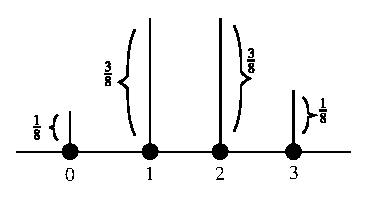
\includegraphics{figure/fig1.eps}}
\smallskip

\underline{table}
\begin{equation*}
\begin{array}{|c|c|c|c|c|}
X & 0 & 1 & 2 & 3\\
\hline
P(X=x) & \dfrac{1}{8} & \dfrac{3}{8} & \dfrac{3}{8} & \dfrac{1}{8}\\
\hline
\end{array}\tag{b}
\end{equation*}
\end{example}
\end{frame}

\begin{frame}
Suppose what to define a new random variable $Y=2X-1$. 

How do we do it?

So how do we define $P(Y=k)$?

Answer - express $Y$ in terms of $X$ and compute so
\begin{align*}
P(Y=k) &= P(2X-1=k)\\[3pt]
       &= P\left(X=\dfrac{k+1}{2}\right)\tag{*}
\end{align*}
The right-hand site is the logical \underline{definition} of the left-hand side. 

But as is often the case in probability it is easier to pretend we know what $P(Y=k)$ means already and then the next two steps are a computation.
\end{frame}

\begin{frame}
So let's compute the $pmf$ of $Y$.

What are the possible values of $Y$?

From (*) $k$ is a possible value of $Y\Leftrightarrow \dfrac{k+1}{2}$ is a possible values of $X$.
$$
\Longleftrightarrow \ \dfrac{k+1}{2}=
\left\{
\begin{array}{c}
0\\
1\\
2\\
3
\end{array}
\right.
\quad \Longleftrightarrow \quad 
Y=
\left\{
\begin{array}{c}
-1\\
1\\
3\\
5
\end{array}
\right.
$$
Note

\centerline{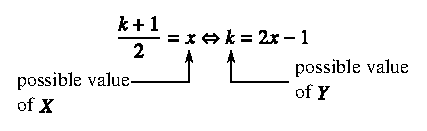
\includegraphics{figure/fig2.eps}}
\end{frame}

\begin{frame}
So the possible values of $Y$ are obtained by applying the function $h(x)=2x-1$ to the possible values of $X$. 

(note $Y=f(X)$).

\medskip
\centerline{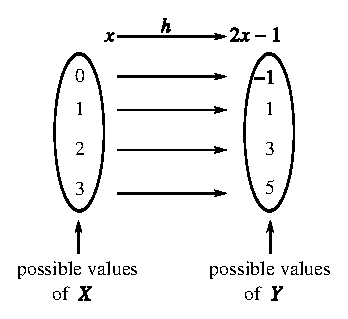
\includegraphics{figure/fig3.eps}}
\medskip

\underline{Just ``push forward'' the values of $X$.}
\end{frame}

\begin{frame}
\begin{nonumexample}[Cont.]
Now we have computed the possible values of $Y$ we need to compute their probabilities. Just repeat what we did
\begin{align*}
P(Y=-1) &= P(2X-1=-1)\\[3pt]
        &= P(X=0)=\frac{1}{8}\\[3pt]
P(Y=1) &= P(2X-1=1)\\[3pt]
       &= P(X=1)=\frac{3}{8}
\end{align*}
Similarly
$$
P(Y=3)=\frac{3}{8}\quad\text{and}\quad P(Y=5)=\frac{1}{8}
$$
\begin{center}
\begin{tabular}{|c|c|c|c|c|}
$X$ & $-1$ & $1$ & $3$ & $5$\\
\hline
$P(Y=y)$ & $\dfrac{1}{8}$ & $\dfrac{3}{8}$ & $\dfrac{3}{8}$ & $\dfrac{1}{8}$\\
\hline
\end{tabular}
\end{center}
\end{nonumexample}
\end{frame}

\begin{frame}
So we have the ``same probabilities'' as before namely $\dfrac{1}{8}$, $\dfrac{3}{8}$, $\dfrac{3}{8}$, $\dfrac{1}{8}$ it is just then are pushed-forward to new locations

\medskip
\centerline{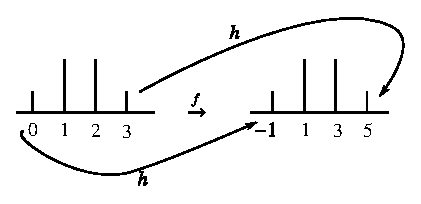
\includegraphics{figure/fig4.eps}}
\end{frame}

\begin{frame}
\begin{example}[Probabilities can ``coalesce'']
There is one tricky point. Several different possible valves of $X$ can push-forward to the same values of $Y$. We now give an example.

Suppose $X$ has proof

\medskip
\centerline{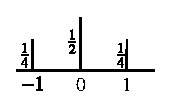
\includegraphics{figure/fig5.eps}}
\smallskip
\end{example}

\begin{nonumproblem}[from on old midterm]
Find a linear change of variable $Y=aX+b$ so that $Y\sim \Bin \left(2,\dfrac{1}{2}\right)$
\end{nonumproblem}
\end{frame}

\begin{frame}
\begin{nonumproblem}[Cont.]
We will make the change of variable $Y=X^{2}$. So what happens when we push forward the three values $-1$, $0$, $1$ by $h(x)=x^{2}$.

We get only the \underline{two} values $0$ and $1$.
\begin{center}
\begin{tabular}{ccc}
$-1$ & $\xrightarrow{h(x)}$ & $1$\\[3pt]
$0$ & $\xrightarrow{\quad~~}$ & $0$\\[3pt]
$1$ & $\xrightarrow{\quad~~}$ & $1$
\end{tabular}
\end{center}
What happens with the corresponding probabilities
$$
P(Y=0)=P(X^{2}=0)=P(X=0)=\dfrac{1}{2}
$$
But
\begin{align*}
P(Y=1) &= P(X^{2}=1)=P(X=1\text{~ or~ } X=-1)\\[3pt]
       &= P((X=1)\cup (X-1))\\[3pt]
       &= P(X=1)+P(X=-1)\\[3pt]
       &= \dfrac{1}{4}+\dfrac{1}{4}=\dfrac{1}{2}
\end{align*}
\end{nonumproblem}
\end{frame}

\begin{frame}
\begin{nonumproblem}[Cont.]
So we set
\begin{center}
\begin{tabular}{|c|c|c|}
$g$ & $0$ & $1$\\[2pt]
\hline
$P(y=9)$ & $\dfrac{1}{2}$ & $\dfrac{1}{2}$\\
\hline
\end{tabular}
\end{center}
So,

\medskip
\centerline{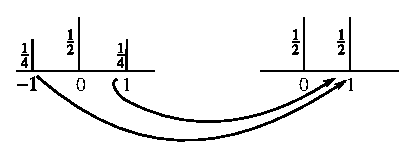
\includegraphics{figure/fig6.eps}}
\smallskip

Think of two masses (probabilities) of mass $\dfrac{1}{4}$ coalesing into a combined mass of $\dfrac{1}{2}$.
\end{nonumproblem}
\end{frame}

\begin{frame}
\myheading{The Expected Value Formula}

If $h(x)$ in the transformation law $Y=h(X)$ is complicated it can be very hard to explicitly compute the $pmf$ of $Y$ Amazingly we can compute the expected value $E(Y)$ using the old proof $P_{X}^{(x)}$ of $X$ according to \underline{Theorem}
\begin{align*}
E(h(X)) &= \sum\limits_{\substack{\text{possible}\\ \text{values of $X$}}} h(x)P_{X}^{(x)}\\[3pt]
        &= \sum\limits_{\substack{\text{possible values}\\ \text{of $X$}}}h(x)P(X=x)
\end{align*}
\end{frame}

\begin{frame}
We will illustrate this with the $pmf$'s of Example \ref{art9-exam1}.

\smallskip

First we compute $E(Y)$ \underline{using the definition of $E(Y)$}. 
\begin{equation*}
\begin{array}{|c|c|c|c|c|}
Y & -1 & 1 & 3 & 5\\
\hline
P(Y=y) & \frac{1}{8} & \frac{3}{8} & \frac{3}{8} & \frac{1}{8}\\
\hline
\end{array}\tag{$\sharp$}
\end{equation*}
\begin{align*}
E(Y) &= \sum\limits_{\substack{\text{possible value}\\ \text{of $Y$}}} y \ P(Y=y)\\[3pt]
     &= (-1)\left(\dfrac{1}{8}\right)+(1)\left(\dfrac{3}{8}\right)+(3)\left(\dfrac{3}{8}\right)+(5)\left(\dfrac{1}{8}\right)\\[3pt]
     &= \dfrac{-1+3+9+5}{8}\\[3pt]
     &= \dfrac{16}{8}=2
\end{align*}
\end{frame}

\begin{frame}
Notice to do the previous computations we needed the table $(\sharp)$ which we computed on page 5.

Now we use the \underline{Theorem}.

So now we use that $Y$ is a function of the random variable $X$ and use the proof of $X$ from the table on page 1.
\begin{equation*}
\begin{array}{|c|c|c|c|c|}
x & 0 & 1 & 2 & 3\\
\hline
P(X=x) & \frac{1}{8} & \frac{3}{8} & \frac{3}{8} & \frac{1}{8}\\
\hline
\end{array}\tag{b}
\end{equation*}
\begin{align*}
E(X) &= \sum\limits_{\substack{\text{possible values}\\ \text{of $X$}}} h(x)P(X=x)\\[3pt]
     &= \sum\limits_{x=0,1,2,3}(2x-1)P(X=x)\\[3pt]
     &= (-1)\left(\dfrac{1}{8}\right)+(1)\left(\dfrac{3}{8}\right)+(3)\left(\dfrac{5}{8}\right)+(5)\left(\dfrac{3}{8}\right)=2
\end{align*}
\end{frame}

\begin{frame}
The most common change of variable is linear $Y=X+b$ so we will give formulas to show how expected value and variance behave under such a change.

\begin{nonumtheorem}
\begin{itemize}
\item[(i)] $E(aX+b)=aE(X)+b$

\item[(ii)] $V(aX+b)=a^{2}V(X)$
\end{itemize}
(so $V(-X)=V(X)$)
\end{nonumtheorem}
\end{frame}

\end{document}


